\documentclass{standalone}
\usepackage{tikz}
\usepackage{tikz-cd}
\usepackage{tikz-3dplot}
\usepackage{pgfplots}
\usepackage{pgffor} % For \foreach loop
\pgfplotsset{compat=newest} % Adjust to your version of pgfplots
\def\Circlearrowleft{\ensuremath{%
		\rotatebox[origin=c]{180}{$\circlearrowleft$}}}
\def\Circlearrowright{\ensuremath{%
		\rotatebox[origin=c]{180}{$\circlearrowright$}}}
\def\CircleArrowleft{\ensuremath{%
		\reflectbox{\rotatebox[origin=c]{180}{$\circlearrowleft$}}}}
\def\CircleArrowright{\ensuremath{%
		\reflectbox{\rotatebox[origin=c]{180}{$\circlearrowright$}}}}
\usetikzlibrary{
	3d, % For 3D drawing
	angles,
	arrows,
	arrows.meta,
	backgrounds,
	bending,
	calc,
	decorations.pathmorphing,
	decorations.pathreplacing,
	decorations.markings,
	fit,
	matrix,
	patterns,
	patterns.meta,
	positioning,
	quotes,
	shadows,
	shapes,
	shapes.geometric
}

\begin{document}
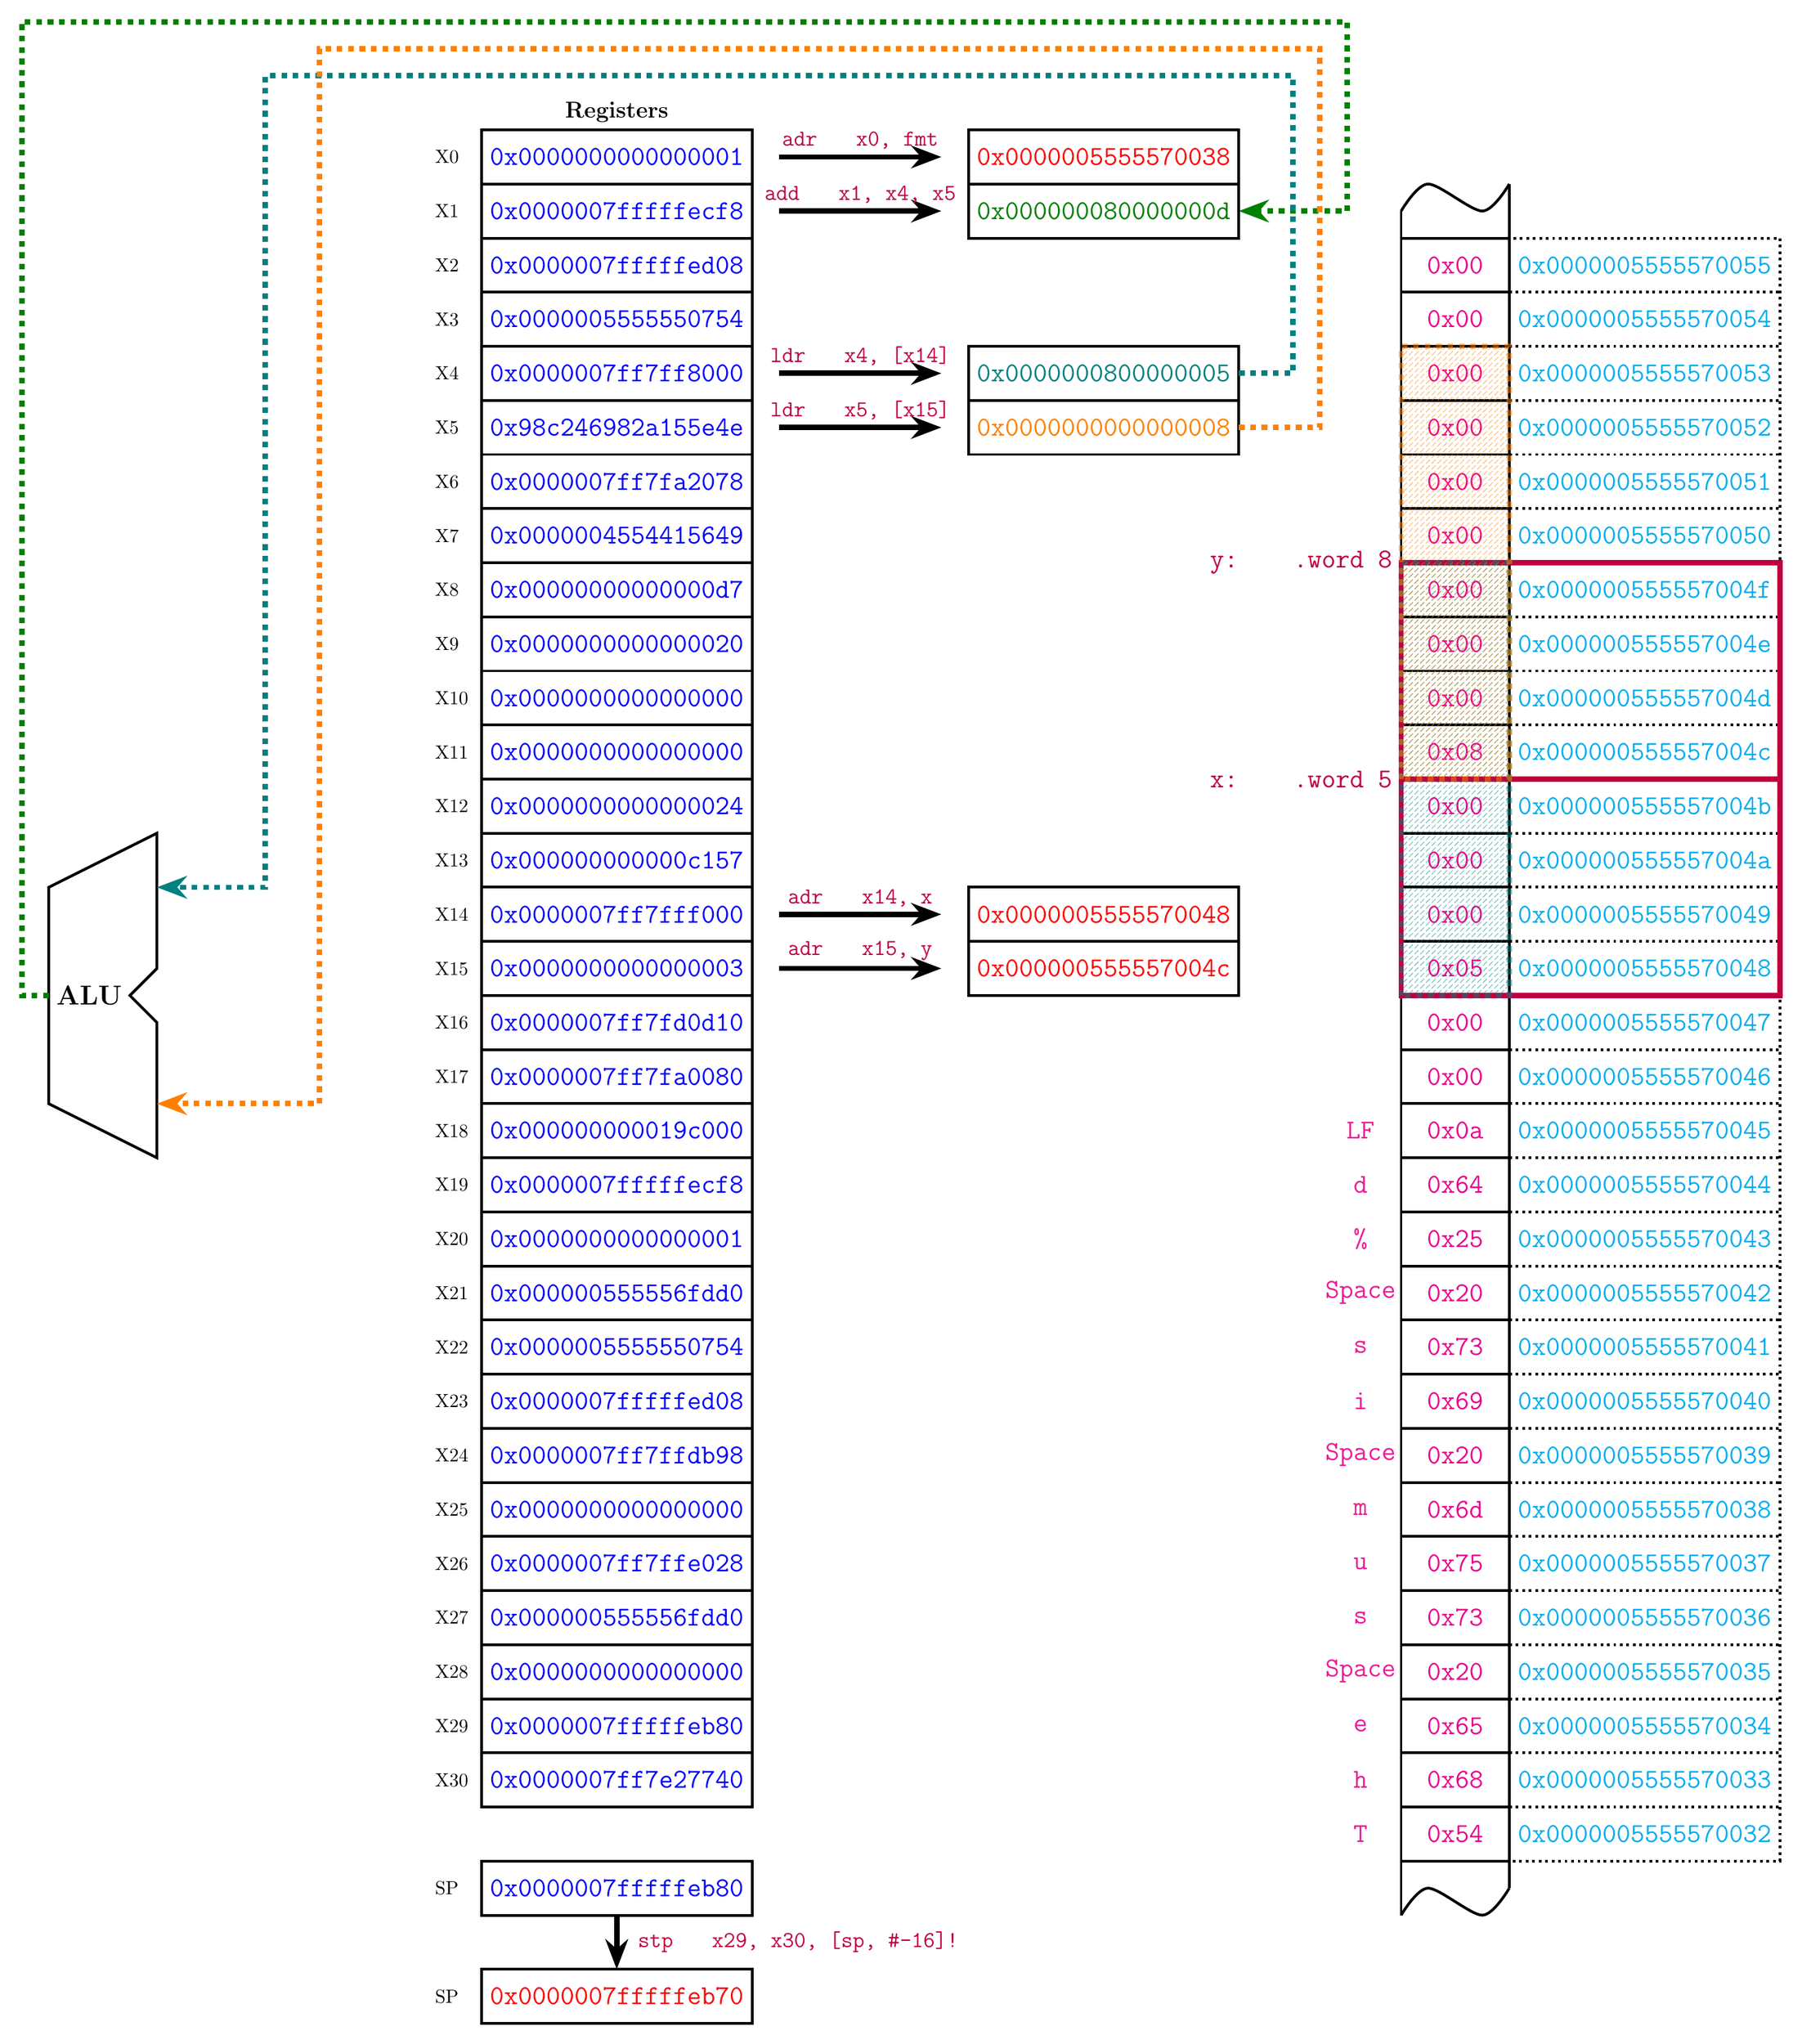
\begin{tikzpicture}[>=Stealth, line width=.5mm]
	\def \x{20}
	\def \y{20}
%	\draw[very thin,color=gray!15,step=.5] (-\x,-\y) grid (\x,\y);
%	
%	\foreach \i in {-\x,...,-2,-1,1,2,...,\x}
%	\draw[gray] (\i,.1)--(\i,-.1) node[below] {$\i$};%x-axis
%	\foreach \i in {-\y,-1,1,1,\y}
%	\draw[gray] (.1,\i)--(-.1,\i) node[left] {$\i$};%y-axis

\begin{scope}[xshift=-7cm]
	\draw[] (-10, -2) -- (-8, -3) -- (-8, -.5) -- (-8.5, 0) -- (-8, .5) -- (-8, 3) -- (-10, 2) -- cycle node[midway, right] {\Large\bf ALU};
	\draw[->, dashed, green!50!black, line width=1mm] (-10, 0) to (-10.5, 0) -- (-10.5, 18) -- (14, 18) -- (14, 14.5) -- (12, 14.5);
%	\draw[->] (-7, 2) to (-8, 2);
%	\draw[->] (-7, -2) to (-8, -2);
\end{scope}

% Processor Core Section
\begin{scope}[xshift=-4cm]
	% Registers section (left side)
	\node[above] at (-2.5, 16) {\large\bf Registers};
	\draw[] (-5, -15) rectangle (0, 16); % Outer box
	\foreach \i in {0, 1, ..., 30} {
		\node[anchor=west] at (-6, 15.5-\i) {X\i};
	}
	\node[anchor=west] at (-6, -16.5) {SP};
	\node[anchor=west] at (-6, -18.5) {SP};
	
	\foreach \i in {15,14,...,-14} {
		\draw (-5,\i) -- (0, \i);
	}
	\draw[] (-5, -17) rectangle (0, -16);
	\draw[->,line width=1mm] (-2.5,-17) to (-2.5,-18);
	\node[right] at (-2.25, -17.5) {\color{purple}\large\ttfamily stp\hspace{.5cm} x29, x30, [sp, \#-16]!};
	\draw[] (-5, -19) rectangle (0, -18);
	
	\def\i{15.5}
	\foreach \j in {
		0x0000000000000001, 0x0000007fffffecf8, 0x0000007fffffed08,
		0x0000005555550754, 0x0000007ff7ff8000, 0x98c246982a155e4e,
		0x0000007ff7fa2078, 0x0000004554415649, 0x00000000000000d7,
		0x0000000000000020, 0x0000000000000000, 0x0000000000000000,
		0x0000000000000024, 0x000000000000c157, 0x0000007ff7fff000,
		0x0000000000000003, 0x0000007ff7fd0d10, 0x0000007ff7fa0080,
		0x000000000019c000, 0x0000007fffffecf8, 0x0000000000000001,
		0x000000555556fdd0, 0x0000005555550754, 0x0000007fffffed08,        
		0x0000007ff7ffdb98, 0x0000000000000000, 0x0000007ff7ffe028,
		0x000000555556fdd0, 0x0000000000000000, 0x0000007fffffeb80,        
		0x0000007ff7e27740
	} {
		\node[blue] at (-2.5, \i) {\Large\texttt{\j}};
		\pgfmathsetmacro{\i}{\i- 1}
		\xdef\i{\i}
	}
	\node[blue] at (-2.5, -16.5) {\Large\texttt{0x0000007fffffeb80}};
	\node[red] at (-2.5, -18.5) {\Large\texttt{0x0000007fffffeb70}};
\end{scope}

\begin{scope}[xshift=5cm]
	% adr x14, x
	\draw[->, line width=1mm] (-8.5, 1.5) to (-5.5,1.5);
	\node[above] at (-7,1.5) {\color{purple}\large\ttfamily adr\hspace{.5cm} x14, x};
	\draw[] (-5, 1) rectangle (0, 2);
	
	\node[red] at (-2.5,1.5) {\Large\ttfamily 0x0000005555570048};
	
	% adr x15, y
	\draw[->, line width=1mm] (-8.5, .5) to (-5.5,.5);
	\node[above] at (-7,.5) {\color{purple}\large\ttfamily adr\hspace{.5cm} x15, y};
	\draw[] (-5, 0) rectangle (0, 1);
	
	\node[red] at (-2.5,.5) {\Large\ttfamily 0x000000555557004c};
	
	% ldr x4, [x14]
	\draw[->, line width=1mm] (-8.5, 11.5) to (-5.5,11.5);
	\node[above] at (-7,11.5) {\color{purple}\large\ttfamily ldr\hspace{.5cm} x4, [x14]};
	\draw[] (-5, 12) rectangle (0, 11);
	
	\node[teal] at (-2.5,11.5) {\Large\ttfamily 0x0000000800000005};
	
	% ldr x5, [x15]
	\draw[->, line width=1mm] (-8.5, 10.5) to (-5.5,10.5);
	\node[above] at (-7,10.5) {\color{purple}\large\ttfamily ldr\hspace{.5cm} x5, [x15]};
	\draw[] (-5, 11) rectangle (0, 10);
	
	\node[orange] at (-2.5,10.5) {\Large\ttfamily 0x0000000000000008};
	
	\draw[teal, ->, dashed, line width=1mm] (0, 11.5) -- (1, 11.5) -- (1, 17) -- (-18,17) -- (-18, 2) -- (-20, 2);
	\draw[orange, ->, dashed, line width=1mm] (0, 10.5) -- (1.5, 10.5) -- (1.5, 17.5) -- (-17,17.5) -- (-17, -2) -- (-20, -2);
	
	% add x1, x4, x5
	\draw[->, line width=1mm] (-8.5, 14.5) to (-5.5,14.5);
	\node[above] at (-7,14.5) {\color{purple}\large\ttfamily add\hspace{.5cm} x1, x4, x5};
	\draw[] (-5, 14) rectangle (0, 15);
	
	\node[green!50!black] at (-2.5,14.5) {\Large\ttfamily 0x000000080000000d};
	
	% adr x0, fmt
	\draw[->, line width=1mm] (-8.5, 15.5) to (-5.5,15.5);
	\node[above] at (-7,15.5) {\color{purple}\large\ttfamily adr\hspace{.5cm} x0, fmt};
	\draw[] (-5, 15) rectangle (0, 16);
	
	\node[red] at (-2.5,15.5) {\Large\ttfamily 0x0000005555570038};
\end{scope}
% Memory section (right side)
\begin{scope}[xshift=8cm]
	% Contents
	\draw[] (0, -16) rectangle (2, 14); % Outer box
	\draw[dotted] (2, -16) rectangle (7, 14); % Outer box
	\foreach \i in {13,12,...,0,-1,-2,...,-15} {
		\draw (0,\i) -- (2, \i);
	}
	% Address
	\foreach \i in {13,12,...,0,-1,-2,...,-15} {
		\draw[dotted] (2,\i) -- (7, \i);
	}
	\draw (0,14) to (0,14.5); \draw (2,14) to (2,15);
	\draw[smooth] plot coordinates {(0,14.5) (.5, 15) (1.5, 14.5) (2,15)};
	\draw (0,-17) to (0,-16); \draw (2,-16) to (2,-16.5);
	\draw[smooth] plot coordinates {(2,-16.5) (1.5, -17) (.5, -16.5) (0,-17)};
	
	\def\i{13.5}
	\foreach \j in {
		0x0000005555570055, 
		0x0000005555570054, 
		0x0000005555570053, 
		0x0000005555570052, 
		0x0000005555570051, 
		0x0000005555570050, 
		0x000000555557004f, 
		0x000000555557004e,
		0x000000555557004d, 
		0x000000555557004c,
		0x000000555557004b,
		0x000000555557004a,
		0x0000005555570049,
		0x0000005555570048,
		0x0000005555570047,
		0x0000005555570046, 
		0x0000005555570045,
		0x0000005555570044,
		0x0000005555570043,
		0x0000005555570042,
		0x0000005555570041,
		0x0000005555570040,
		0x0000005555570039,
		0x0000005555570038,
		0x0000005555570037,
		0x0000005555570036,
		0x0000005555570035,
		0x0000005555570034,
		0x0000005555570033,
		0x0000005555570032
	} {
		\node[cyan] at (4.5, \i) {\Large\texttt{\j}};
		\pgfmathsetmacro{\i}{\i- 1}
		\xdef\i{\i}
	}

	\def\i{-15.5}
	\foreach \j in {
		0x54, 0x68, 0x65, 0x20,
		0x73, 0x75, 0x6d, 0x20,
		0x69, 0x73, 0x20, 0x25,
		0x64, 0x0a, 0x00, 0x00,
		0x05, 0x00, 0x00, 0x00,
		0x08, 0x00, 0x00, 0x00,
		0x00, 0x00, 0x00, 0x00,
		0x00, 0x00
	} {
		\node[magenta] at (1, \i) {\Large\texttt{\j}};
		\pgfmathsetmacro{\i}{\i+ 1}
		\xdef\i{\i}
	}

	\draw[purple, line width=1mm] (7, 0) rectangle (0, 4) node[left] {\Large\ttfamily x:\hspace{.5cm} .word 5};
	\draw[purple, line width=1mm] (7, 4) rectangle (0, 8) node[left] {\Large\ttfamily y:\hspace{.5cm} .word 8};
	
	\draw[line width=1mm, dashed, color=teal, pattern=north east lines,pattern color=teal, opacity=.5] (0,0) rectangle (2,8);
	
	\draw[line width=1mm, dashed, color=orange, pattern=north east lines,pattern color=orange, opacity=.5] (0,4) rectangle (2,12);

	\node[magenta!90] at (-.75, -15.5) {\Large\ttfamily T};
	\node[magenta!90] at (-.75, -14.5) {\Large\ttfamily h};
	\node[magenta!90] at (-.75, -13.5) {\Large\ttfamily e};
	\node[magenta!90] at (-.75, -12.5) {\Large\ttfamily Space};
	\node[magenta!90] at (-.75, -11.5) {\Large\ttfamily s};
	\node[magenta!90] at (-.75, -10.5) {\Large\ttfamily u};
	\node[magenta!90] at (-.75, -9.5) {\Large\ttfamily m};
	\node[magenta!90] at (-.75, -8.5) {\Large\ttfamily Space};
	\node[magenta!90] at (-.75, -7.5) {\Large\ttfamily i};
	\node[magenta!90] at (-.75, -6.5) {\Large\ttfamily s};
	\node[magenta!90] at (-.75, -5.5) {\Large\ttfamily Space};
	\node[magenta!90] at (-.75, -4.5) {\Large\ttfamily \%};
	\node[magenta!90] at (-.75, -3.5) {\Large\ttfamily d};
	\node[magenta!90] at (-.75, -2.5) {\Large\ttfamily LF};
\end{scope}
\end{tikzpicture}
\end{document}
